\section{Implementation}
We implemented the techniques and processes described in previous sections on Android platform\cite{webandroid} as a zoomable video player. The architecture of the player is depicted as figure below.

\begin{figure}
\centering
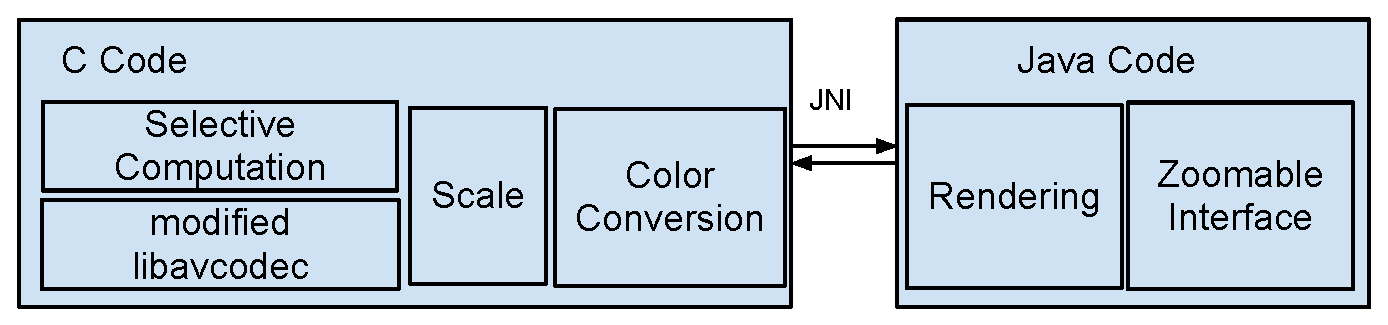
\includegraphics[height=1.8cm]{playernew.eps}
\caption{Zoomable Video Player Implementation}
\end{figure}
Based on the open source MPEG4 SP codec from libavcodec of ffmpeg 0.7\cite{webffmpeg}, we added the selective decoding functions. At the time of implementation, the ffmpeg codec was not optimized to run on Android platform, especially the scale and color conversion process. We adopted the code from another two open source projects, with scale from libyuv\cite{weblibyuv} and color conversion from Google Chromimum project\cite{webchromium}. 

We implemented the rendering and zoomable interface in Java with Android SDK. The gesture detector detects a user's pinch or pan gesture, and translates the gesture detected as zoom scale and pan scale. We then compute a ROI from these scales based on what user can see on the phone screen. 
